\section{Experiments}

Experiments are done with two agent based models in three regions with different population sizes. Number of agents in each of the region are as follows: Rappahannock county has 2495 agents, San Diego has 12925 agents, Shenandoah Valley Region (SVR) has 138043 agents.


Both the agent-based diffusion models simulate the number of households adopting rooftop solar.
The model presented in Section \ref{virginia_model} is used for Rappahannock county in Virginia and Shenandoah Valley Region in Virginia. 
The model presented in Section \ref{san-diego-model} is used for San Diego.
In order to facilitate comparison between the 2 ABMs, we choose to explore the common parameters in both the models: NPV and X1Mile.

Before learning the decision boundary that separates the low and high adoptions for the three regions, we need to set the parameter extents of the search space, $STDEV-THRESHOLD$ for boundary point condition, and $MEAN-THRESHOLD$ for labeling points evaluated in the search space. Diffusion model outputs are examined for points across the diagonal of an arbitrary parameter space.

\begin{figure}
    \centering
    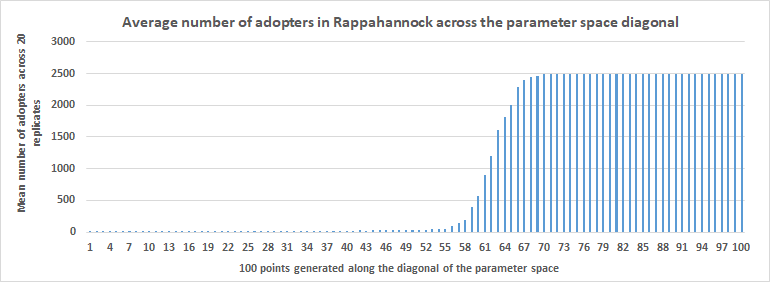
\includegraphics{AAMAS20Template-submission/figures/rapp-diag-mean1.png}
    \caption{Diagonal Mean <ADD MORE>}
    \label{fig:}
\end{figure}

\begin{figure}
    \centering
    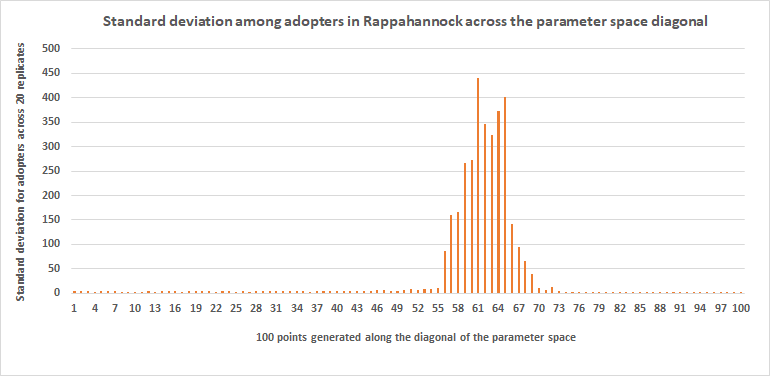
\includegraphics{AAMAS20Template-submission/figures/rapp-diag-stdev1.png}
    \caption{Diagonal Stdev <ADD MORE>}
    \label{fig:}
\end{figure}

\begin{figure}
\begin{subfigure}{.25\textwidth}
  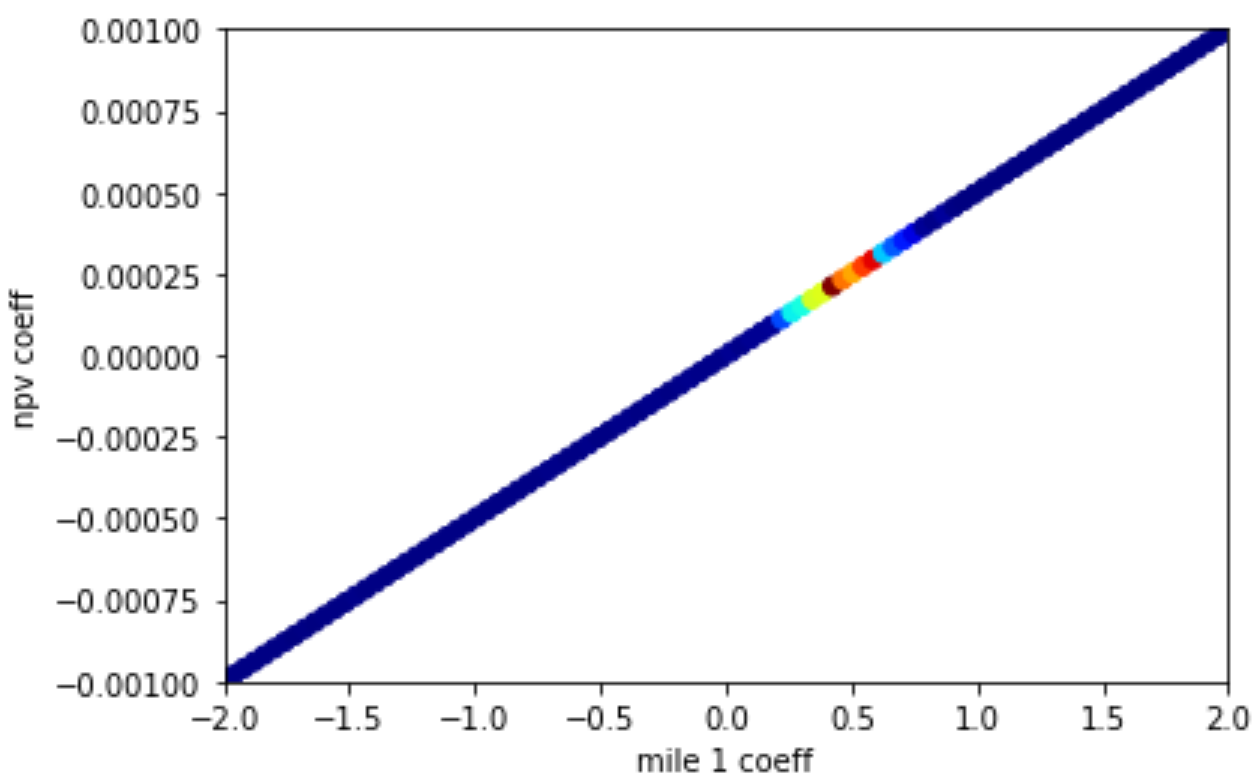
\includegraphics[height=3cm,width=4cm]{AAMAS20Template-submission/figures/rapp100diagstdev.png}
    \caption{Diagonal Stdev <ADD MORE>}
  \label{fig:sub1}
\end{subfigure}%
\begin{subfigure}{.25\textwidth}
  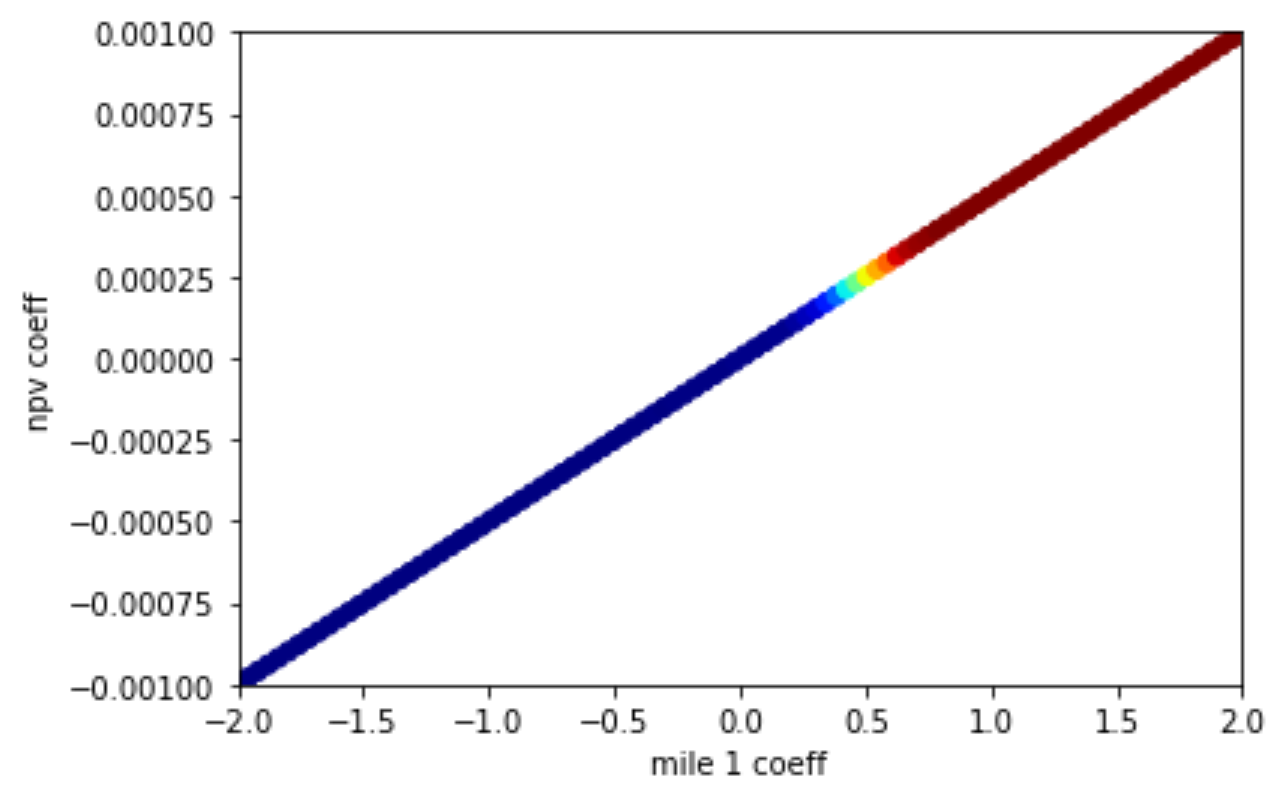
\includegraphics[height=3cm,width=4cm]{AAMAS20Template-submission/figures/rapp100diagmean.png}
  \caption{Diagonal Mean <ADD MORE>}
  \label{fig:sub2}
\end{subfigure}
\caption{A figure with two subfigures}
\label{fig:test}
\end{figure}

\begin{comment}
\begin{figure}
    \centering
    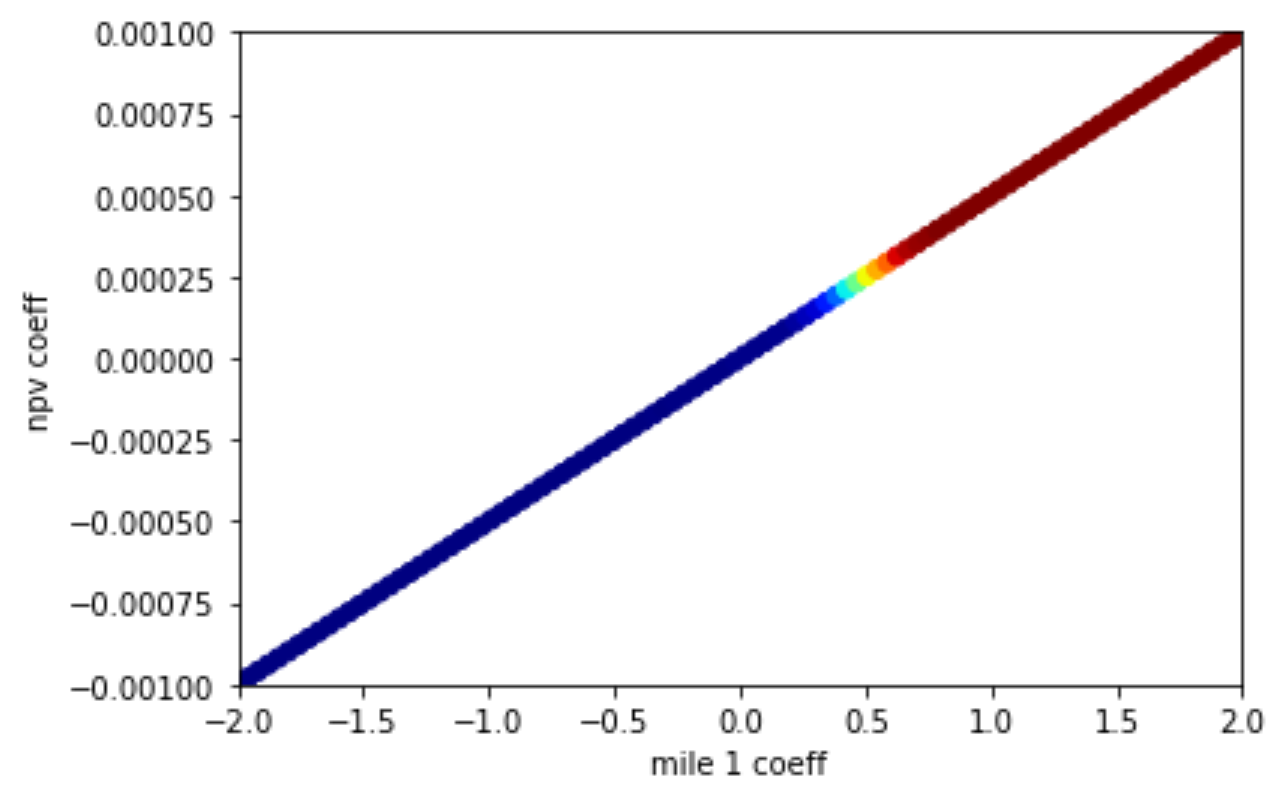
\includegraphics[height=3cm,width=4cm]{AAMAS20Template-submission/figures/rapp100diagmean.png}
    \caption{Diagonal Mean <ADD MORE>}
    \label{fig:}
\end{figure}

\begin{figure}
    \centering
    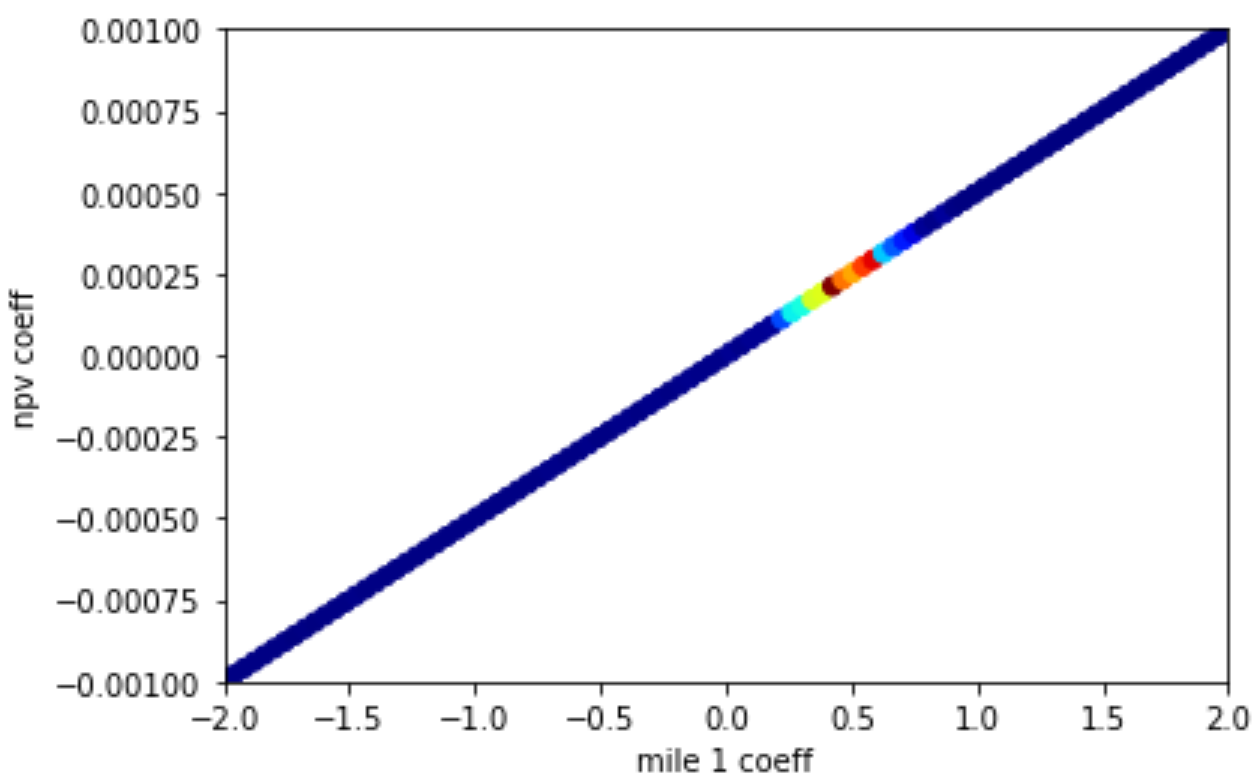
\includegraphics[height=3cm,width=4cm]{AAMAS20Template-submission/figures/rapp100diagstdev.png}
    \caption{Diagonal Stdev <ADD MORE>}
    \label{fig:}
\end{figure}
\end{comment}

{\color{magenta} Q for Samarth: Should we give the mean and stdev thresholds for each region?}

In all the experiment settings, the diffusion model results are averaged over 20 replicates to calculate mean and standard deviation. 
%If time out happens then we discard the point or process how many every replicates are completed.

Two types of approaches are used to find a start point for binary search. The first set of endpoints is chosen to be the diagonal of the parameter search space. From the next round, points are chosen intelligently by exploiting the knowledge of $boundaryPoints$ and $evaluatedPoints$.
First Approach:
Use SVM linear classifier and generate boundary points around the SVM linear boundary.
Choose one point from this set that is far away from points in evaluatedPoints and boundaryPoints obtained at that point in time.
Second approach:
Use Random Forest to train intermediate evaluatedPoints after a boundary point is found. Then choose points that have equal ratio of neighbors with opposite labels. Choose one point from this set that is far away from points in evaluatedPoints and boundaryPoints obtained at that point in time.

